The task was created because the customers expressed concern for the reactiveness of the PictoSearch application, it sometimes felt slow and customers said it felt like nothing was happening.
It is important that responses from a mobile application happen somewhat quickly, as mentioned in~\cite{Roto:2005:NNF:1062745.1062747}, if an application takes more than 4 seconds to load or respond then other feedback than visual should be used.
\kim{It is like this argument was cut short. What should the visual feedback be used for? What would other feedback mechanisms do? I can guess the answer but you should write the entire point not just supply hints.}
Therefore it is decided that almost instantaneous feedback\kim{Can you be a bit more precise, how fast is almost instantaneous feedback? It should be clear what the goal is and why this goal was chosen.} is important such that the users feel like the application is processing the inputs quickly and effective.
This resulted in wanting a change of when calls were made in the PictoSearch application.\kim{rephrase last sentence.}

The current version\todo{Er det forvirende at skrive current version når det er en kontinuer historie? Er det klart at der menes den udgave lavet af de tidligere GIRAF projekter? - Troels}\todo{Kim: Det er tydeligt at forstå hvad der menes.} of the PictoSearch application searches whenever the uses touches\kim{press?} the search button on either the keyboard or on the GUI of the application.
The search button is located in the middle of the screen, to the left of the search field as can be seen on \myref{fig:screenshot_startup}.
\begin{figure}[h]
    \centering
    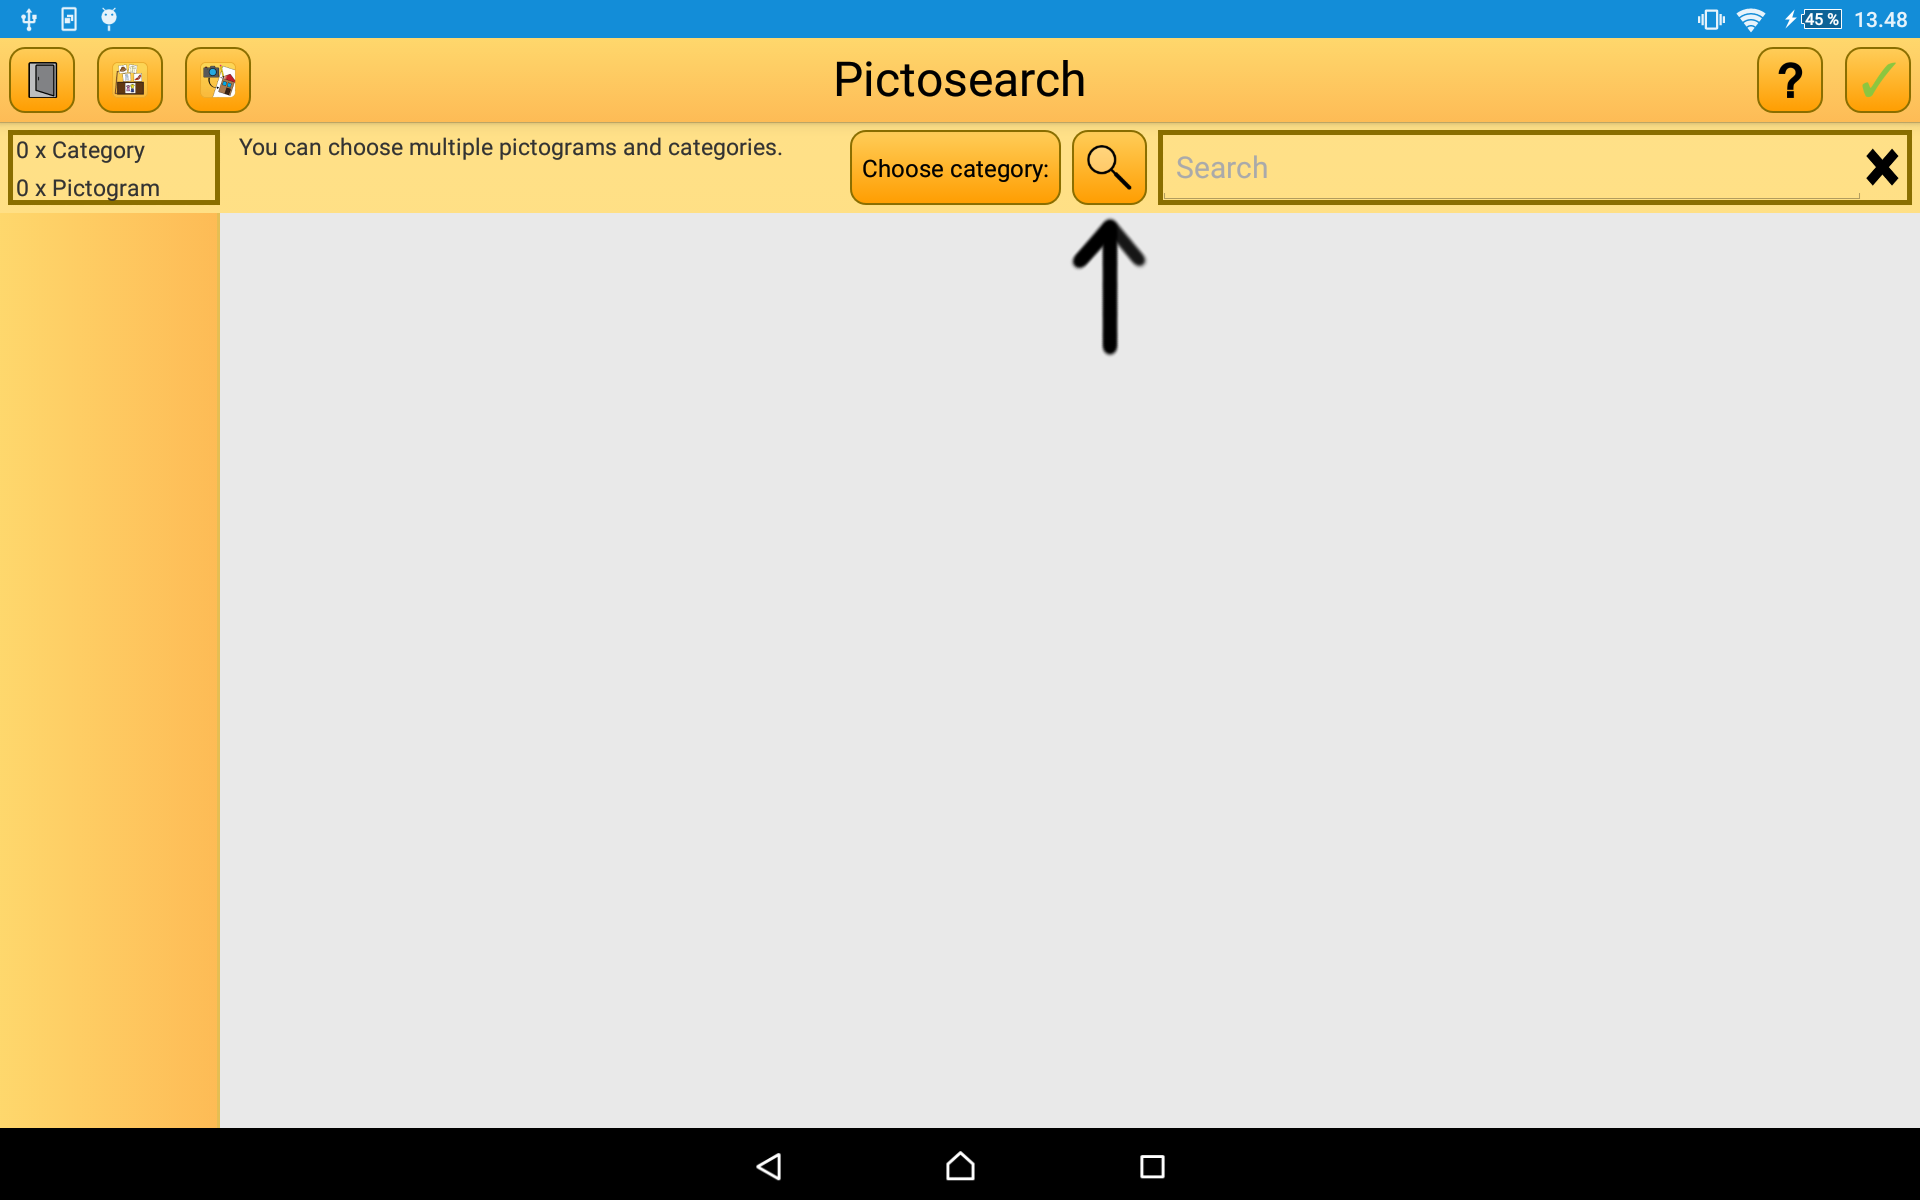
\includegraphics[width=0.8\textwidth]{figures/img/screenshots/old_startup.png}
    \caption{Screenshot of the initial view presented to the user when launching PictoSearch.}\label{fig:screenshot_startup}
\end{figure}
\kim{Maybe highlight it on the screenshot}

\begin{figure}[h]
    \centering
    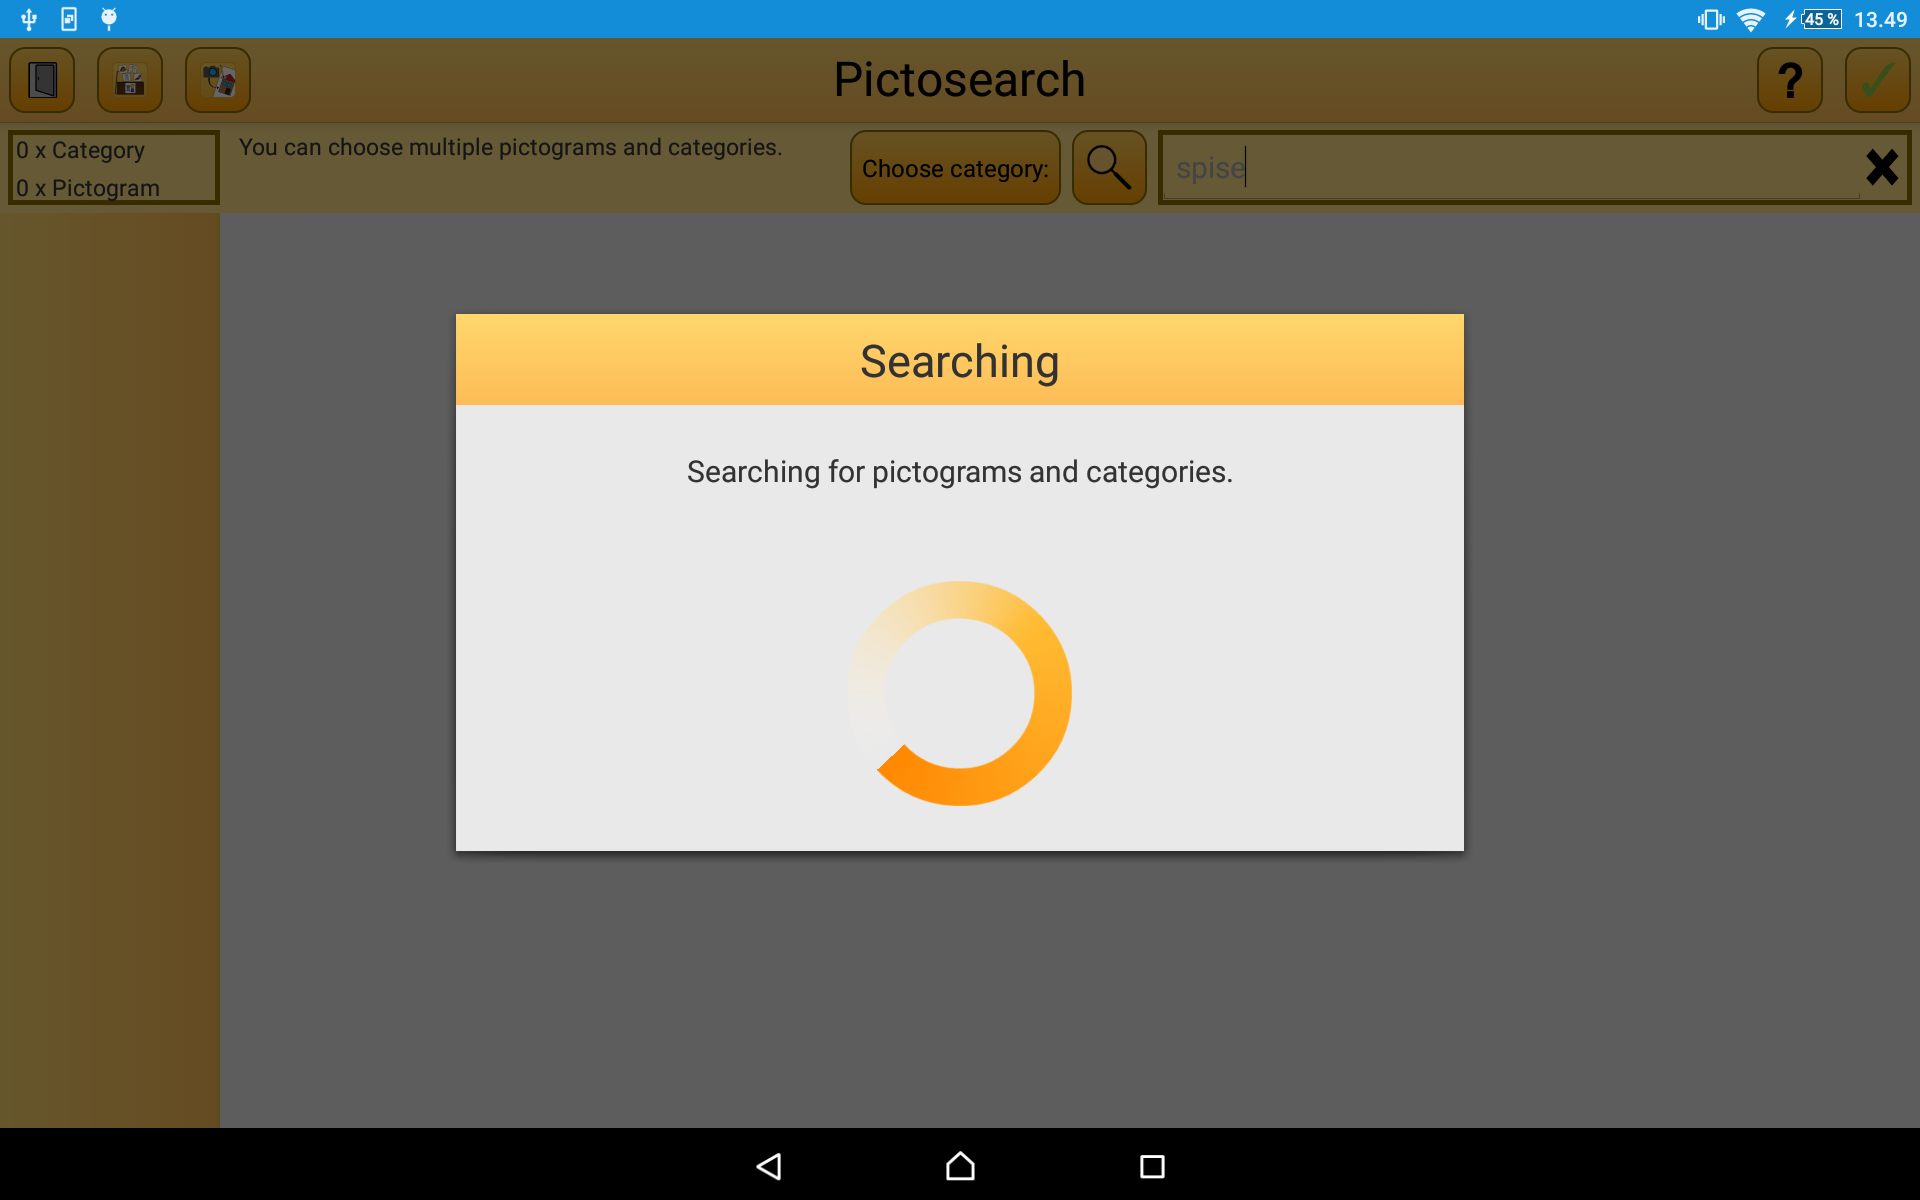
\includegraphics[width=0.8\textwidth]{figures/img/screenshots/old_dialog.png}
    \caption{Screenshot of the search spinner shown while searching in PictoSearch.}\label{fig:screenshot_searchspinner}
\end{figure}
This has been changed such that a search happens whenever the text in the searchfield is changed.
Instead of the big slow search spinner which can be seen on \myref{fig:screenshot_searchspinner}, a new smaller text message is instead displayed which tells the user that the application is searching and what is is searching for. 
This search does not remove the software keyboard from the view, neither does it make you unable to type.
This is possible because the search is implemented as an async task, because of this any new search is queued behind the current search query.
This change is implemented by calling \texttt{AsyncTask.cancel()}, which cancels the ongoing search call and makes it possible to start a new call immediately, with the updated search string.
\kim{I cant help but thinking that this feature have a name, I suggest that you find out what it is called and start using that term.}
Because of this anytime a keystroke is made on the keyboard something should happen on the display other than simply filling out the search-field, be it a text message explaining what is being searched for, or be it the resulting pictograms returned from the search.
\kim{So when is what displayed? please elaborate.}
This means that there is near instantaneous feedback for the user, which should give the feeling that the application is reacting to what the user is doing, and it does no longer feels like nothing is happening.
\kim{Make sure to test if this have the required effect. There is a high probability that the censor that will be at you exam is very interested in GUI and test of these. So make sure that stuff like this is done by the book. Unfortunately then I have limited knowledge of this area.}

The search button can still be used, and will bring up the old search spinner as usually, but the button has been moved from the middle of the display to the right side of the display as can be seen on \myref{fig:screenshot_newstartup}.
This is a better fit as it resembles other common search engines such as Google Search, and it is also the recommended way to display a search-field according to the Niels Norman Group\footnote{https://www.nngroup.com/articles/magnifying-glass-icon/}.
\kim{It would also be easy to find the design principle that says that it is a good thing to use ``structures'' that people recognize. Remember that the theory is very important when doing GUI stuff.}
It can also be seen on \myref{screenshot_newUI} that the cancel search button is only shown when there is actually something to remove from the search field, this removes the clutter of information otherwise produced from the old view.
\kim{I think that the structure of this section is a bit off. First there should be an analysis, what is the problem: No/slow user feedback, Search button is difficult to find (I assume that this is a problem identified by some users), cancel/delete is there when field is blank. Then we describe(design) possible solutions and discuss why they are good/ bad solutions. Choose the best solution and then, if it interesting, show the implementation of the solution (might be sufficient with screenshots.) }

\begin{figure}[h]
    \centering
    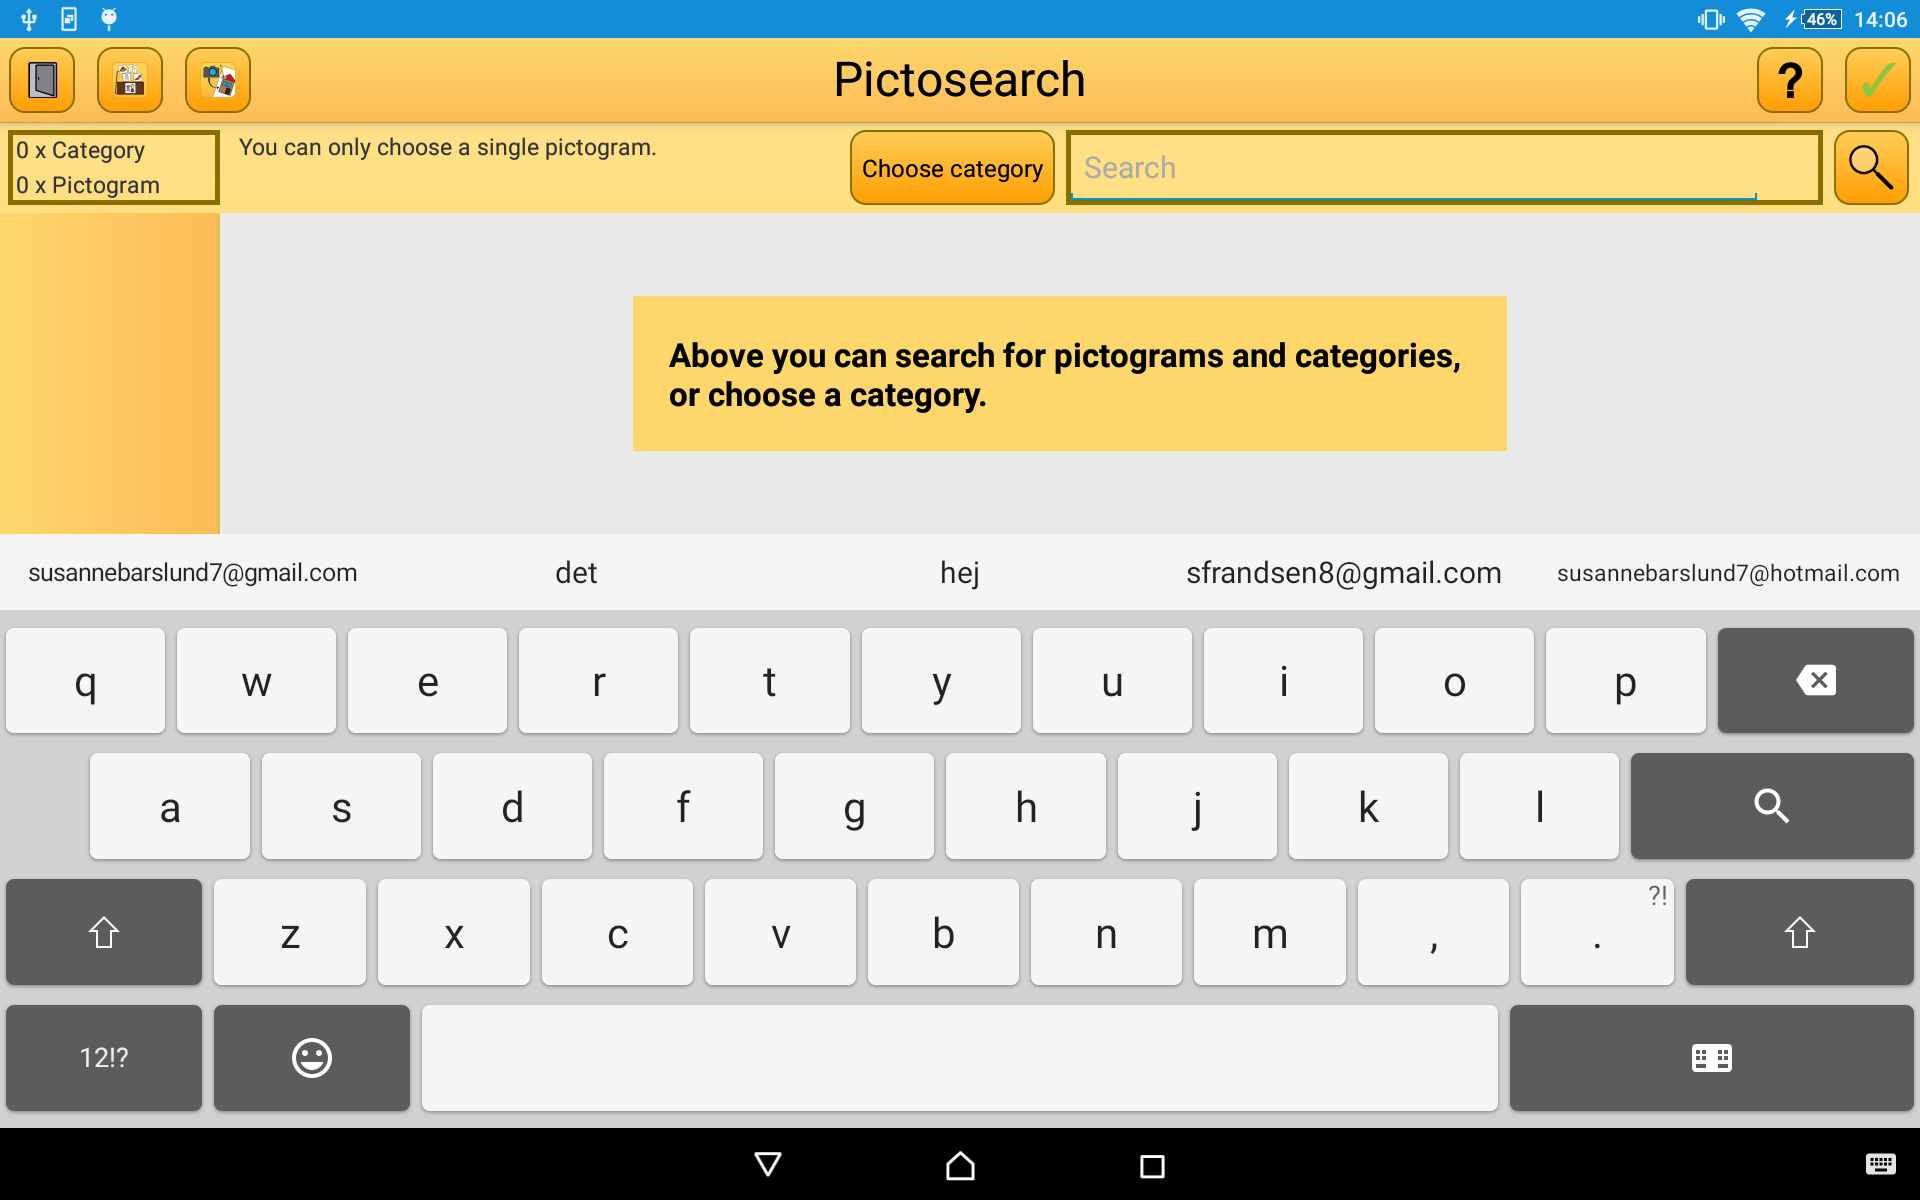
\includegraphics[width=0.8\textwidth]{figures/img/screenshots/new_startup.png}
    \caption{Screenshot of the new initial view in PictoSearch.}\label{fig:screenshot_newstartup}
\end{figure}

\paragraph{Initial view}
\kim{What dies this have to do with responsive search? }
Another change made to PictoSearch involves a task, which describes a need for modifications to be made to the initial view;\kim{instead of describe that there is some mysterious task that have some description, then just reference the tasks name, it is explained two pages above this. Please rephrase.} This is the view that is presented to a user when launching PictoSearch.
In the current version, the user is presented with no useful information in the initial view as seen in \myref{fig:screenshot_startup}. \kim{Try to be more precise, information is not a very descriptive word, it can be anything. Describe in more detail what the problem actually is (analysis)}
Initially this task asked for the showing of somewhat random pictograms in the initial view\kim{This sentence is very informal and does not belong in a bachelor report. Please use more formal and precise language.}, however we suspected that users might get confused by this, and believe that the pictograms shown were the only pictograms available in PictoSearch; therefore we simplified the task to assist the user in using PictoSearch. \kim{It is a problem that the task describes a solution rather then a problem. It it should not be necessary that you change a task because you have designed a good solution to the problem.}
As the aim of the workflow\kim{what workflow? if there is a pictosearch workflow then remember to describe it or reference to a place where it is described.} which involves PictoSearch is to search for pictograms, we set out to reduces the number of actions needed for such an operation. \kim{Why is it a good solution to reduce the number of action that user need to do a good solution to the problem? I see no correlation between this solution and the problem.} 
Furthermore we want to present some descriptive information to the user at any given time, such that it is clear what he or she should do to advance in the searching.
The first change\kim{If there is a first change then I assume that there will be more the one change, no second change is described.} is that the keyboard is forced to appear on the screen when launching PictoSearch, along with giving focus to the search field; this enables the user to start searching right away without having to press anything.
This new initial view, which also includes added informative text can be seen on \myref{fig:screenshot_newstartup}
\kim{Like the section above then this section suffers from structural problem. Try to follow the analyze, design, implement model/structure}
